\chapter{Source Code}

I verify that I am the sole author of the programs contained in this folder, except where explicitly stated to the contrary.

The source code history is also available on GitHub
\begin{enumerate}
    \item Web application: \url{https://github.com/vladstoick/fyp}
    \item Library: \url{https://github.com/vladstoick/fyp_sql_assess}
    \item Parser fork: \url{https://github.com/vladstoick/sql-parser}. In addition the parser is also published on RubyGems \url{https://rubygems.org/gems/sql-parser-vlad}.
\end{enumerate}

The first three sections of this chapter introduce each part of the code, with the next 3 sections presenting the code.

\section{Grading library}

A good way to navigate the source code is to start in the assessor class defined in \path{lib/sql_assess/assesor.rb}. The assessor is the public interface of the library.


\begin{tabularx}{\textwidth}{|X|X|}
    \hline
    \textbf{File} & \textbf{Description} \\\hline
    \endhead
    \path{Gemfile} & Dependencies for library (no dependency listed here as dependencies for ruby gems are pulled from the gem spec) \\\hline
    \path{LICENSE.txt} & MIT License of repository \\\hline
    Rakefile & Defines the rake task of the library as the test spec. A rake task in Ruby is a command that can be executed. \\\hline
    \path{sql_assess.gemspec} & Defines the proprieties of the gem: name, author, licence, and dependencies. \\\hline
    \path{Gemfile.lock} & Defines the versions of dependencies currently installed. When the library is installed it will use these versions. \\\hline
    \path{codecov.yml} & Configuration for codecov \\\hline
    \path{lib/sql_assess.rb} & Defines the namespace of the library and includes all the main sub classes \\\hline
    \path{lib/sql_assess/assesor.rb} & Implementation of \path{Assesor} \\\hline
    \path{lib/sql_assess/data_extractor.rb} & Implementation of \path{DataExtractor} \\\hline
    \path{lib/sql_assess/database_connection.rb} & Implementation of \path{DatabaseConnection} \\\hline
    \path{lib/sql_assess/error.rb} & Definition of various errors from the library \\\hline
    \path{lib/sql_assess/query_attribute_extractor.rb} & Implementation of \path{QueryTransformer} which extracts all attributes from queries \\\hline
    \path{lib/sql_assess/query_comparator.rb} & Implementation of \path{QueryComparator} which compares the results of two queries \\\hline
    \path{lib/sql_assess/query_comparison_result.rb} & Implementation of \path{QueryComparisonResult} which represents the final result of an assessment \\\hline
    \path{lib/sql_assess/query_transformer.rb} & Implementation of \path{QueryTransformer} which transforms queries \\\hline
    \path{lib/sql_assess/runner.rb} & Implementation of \path{Runner} which runs various queries \\\hline
    \path{lib/sql_assess/version.rb} & Defines the current version of the library \\\hline
    \path{lib/sql_assess/graders/base.rb} & Implementation of \path{Graders::Base} which provides a base for all graders \\\hline
    \path{lib/sql_assess/graders/**.rb} & All files in this folder define a grader for a component. They all inherit from \path{Graders::Base} \\\hline
    \path{lib/sql_assess/parsers/base.rb} & Implementation of \path{Parsers::Base} which provides a base for all parsers \\\hline
    \path{lib/sql_assess/parsers/**.rb} & All files in this folder define a parser for a component. They all inherit from \path{Parsers::Base} \\\hline
    \path{lib/sql_assess/transformers/base.rb} & Implementation of \path{Transformers::Base} which provides a base for all parsers \\\hline
    \path{lib/sql_assess/transformers/all_columns.rb} & Implementation of \path{Transformers::AllColumns} which transforms \path{*} to all columns \\\hline
    \path{lib/sql_assess/transformers/from_subquery.rb} & Implementation of \path{Transformers::FromSubquery} which canonicalizes the queries from the \path{FROM} clause \\\hline
    \path{lib/sql_assess/transformers/ambigous_columns/base.rb} & Implementation of \path{Transformers::AmbigousColumns::Base} which provides a base for all ambiguous columns transformers \\\hline
    \path{lib/sql_assess/transformers/ambigous_columns/**.rb} & All files in this folder define an ambiguous column transformer for a component. They all inherit from \path{Transformers::AmbigousColumns::Base} \\\hline
    \path{lib/sql_assess/transformers/between_predicate/base.rb} & Implementation of \path{Transformers::BetweenPredicate::Base} which provides a base for all between predicate transformers \\\hline
    \path{lib/sql_assess/transformers/between_predicate/**.rb} & All files in this folder define an between predicate transformer for a component. They all inherit from \path{Transformers::BetweenPredicate::Base} \\\hline
    \path{lib/sql_assess/transformers/comparison_predicate/base.rb} & Implementation of \path{Transformers::ComparisonPredicate::Base} which provides a base for all comparison predicate transformers \\\hline
    \path{lib/sql_assess/transformers/comparison_predicate/**.rb} & All files in this folder define an comparison predicate transformer for a component. They all inherit from \path{Transformers::ComparisonPredicate::Base} \\\hline
    \path{lib/sql_assess/transformers/equivalent_columns/base.rb} & Implementation of \path{Transformers::EquivalentColumns::Base} which provides a base for all equivalent columns transformers \\\hline
    \path{lib/sql_assess/transformers/equivalent_columns/**.rb} & All files in this folder define an equivalent column transformer for a component. They all inherit from \path{Transformers::EquivalentColumns::Base} \\\hline
    \path{lib/sql_assess/transformers/not/base.rb} & Implementation of \path{Transformers::Not::Base} which provides a base for all not predicate transformers \\\hline
    \path{lib/sql_assess/transformers/not/**.rb} & All files in this folder define an not predicate transformer for a component. They all inherit from \path{Transformers::Not::Base} \\\hline
    \path{spec/spec_helper.rb} & RSpec configuration \\\hline
    \path{spec/sql_assess_namespace.rb} & Version test \\\hline
    \path{spec/fixtures/**.yml} & Integration tests data \\\hline
    \path{spec/tests/**/class_name_spec.yml} & Tests that test the \path{class_name} \\\hline
\end{tabularx}

\section{Web application}

The web application follows a pattern similar to an MVC framework (views, models, controllers). The rails app contains many folders by default, but the most important ones are:
\begin{tabularx}{\textwidth}{|X|X|}
    \hline
    \textbf{File} & \textbf{Description} \\\hline
    \endhead
    \path{Gemfile} & Dependencies for the web application \\\hline
    \path{Gemfile.lock} & Defines the versions of dependencies currently installed. When the web application is installed it will use these versions. \\\hline
    \path{LICENSE.txt} & MIT License of repository \\\hline
    \path{package.json} & Javascript dependencies \\\hline
    \path{yarn.lock} & Javascript dependencies fixed version \\\hline
    \path{db/seeds.rb} & Initial data inserted in the database \\\hline
    \path{db/schema.rb} & Schema of the database \\\hline
    \path{db/migrate/**.rb} & Database migrations \\\hline
    \path{app/controllers/**.rb} & Controllers \\\hline
    \path{app/models/**.rb} & Models \\\hline
    \path{app/views/**.rb} & Views \\\hline
    \path{app/policies/**.rb} & Policies \\\hline
    \path{app/javascript/packs/**.js} & Javascript code \\\hline
    \path{app/javascript/styles/**.scss} & SCSS code \\\hline
    \path{app/spec/features/**.rb} & Integration tests \\\hline
    \path{app/spec/models/**.rb} & Unit tests for models \\\hline
    \path{app/spec/requests/**.rb} & Unit tests for controllers \\\hline
    \path{app/spec/factories/**.rb} & Factories for models \\\hline
\end{tabularx}

\section{Sql parser}

As the sql-parser is an existing library, this section will only include the added feature in the form of a diff file. This is to clearly indicate what work was done by this project. For the full code please refer to the GitHub repo or the source code zip. The zip code will contain the full source code.

\section{Code for library}
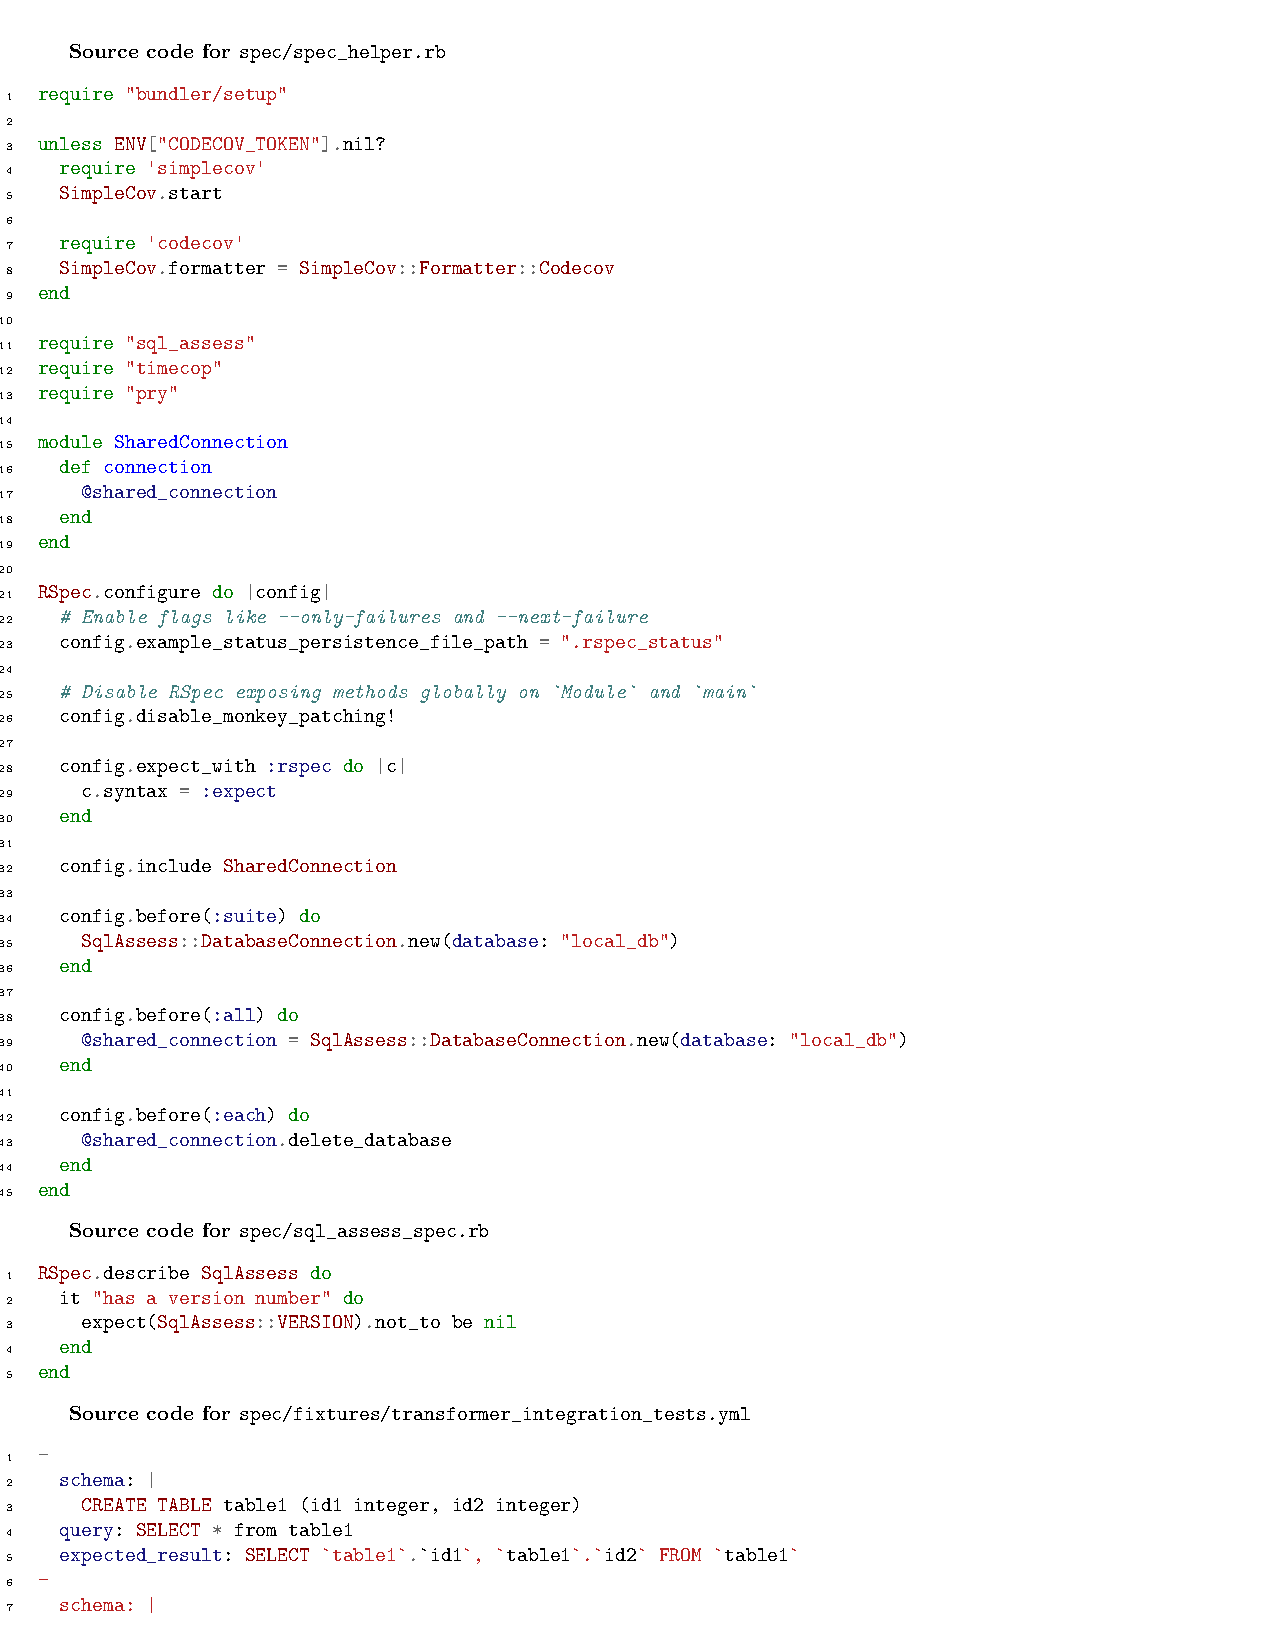
\includepdf[pages=1-122]{Appendices/sourcecodelibrary.pdf}
\section{Code for web app}
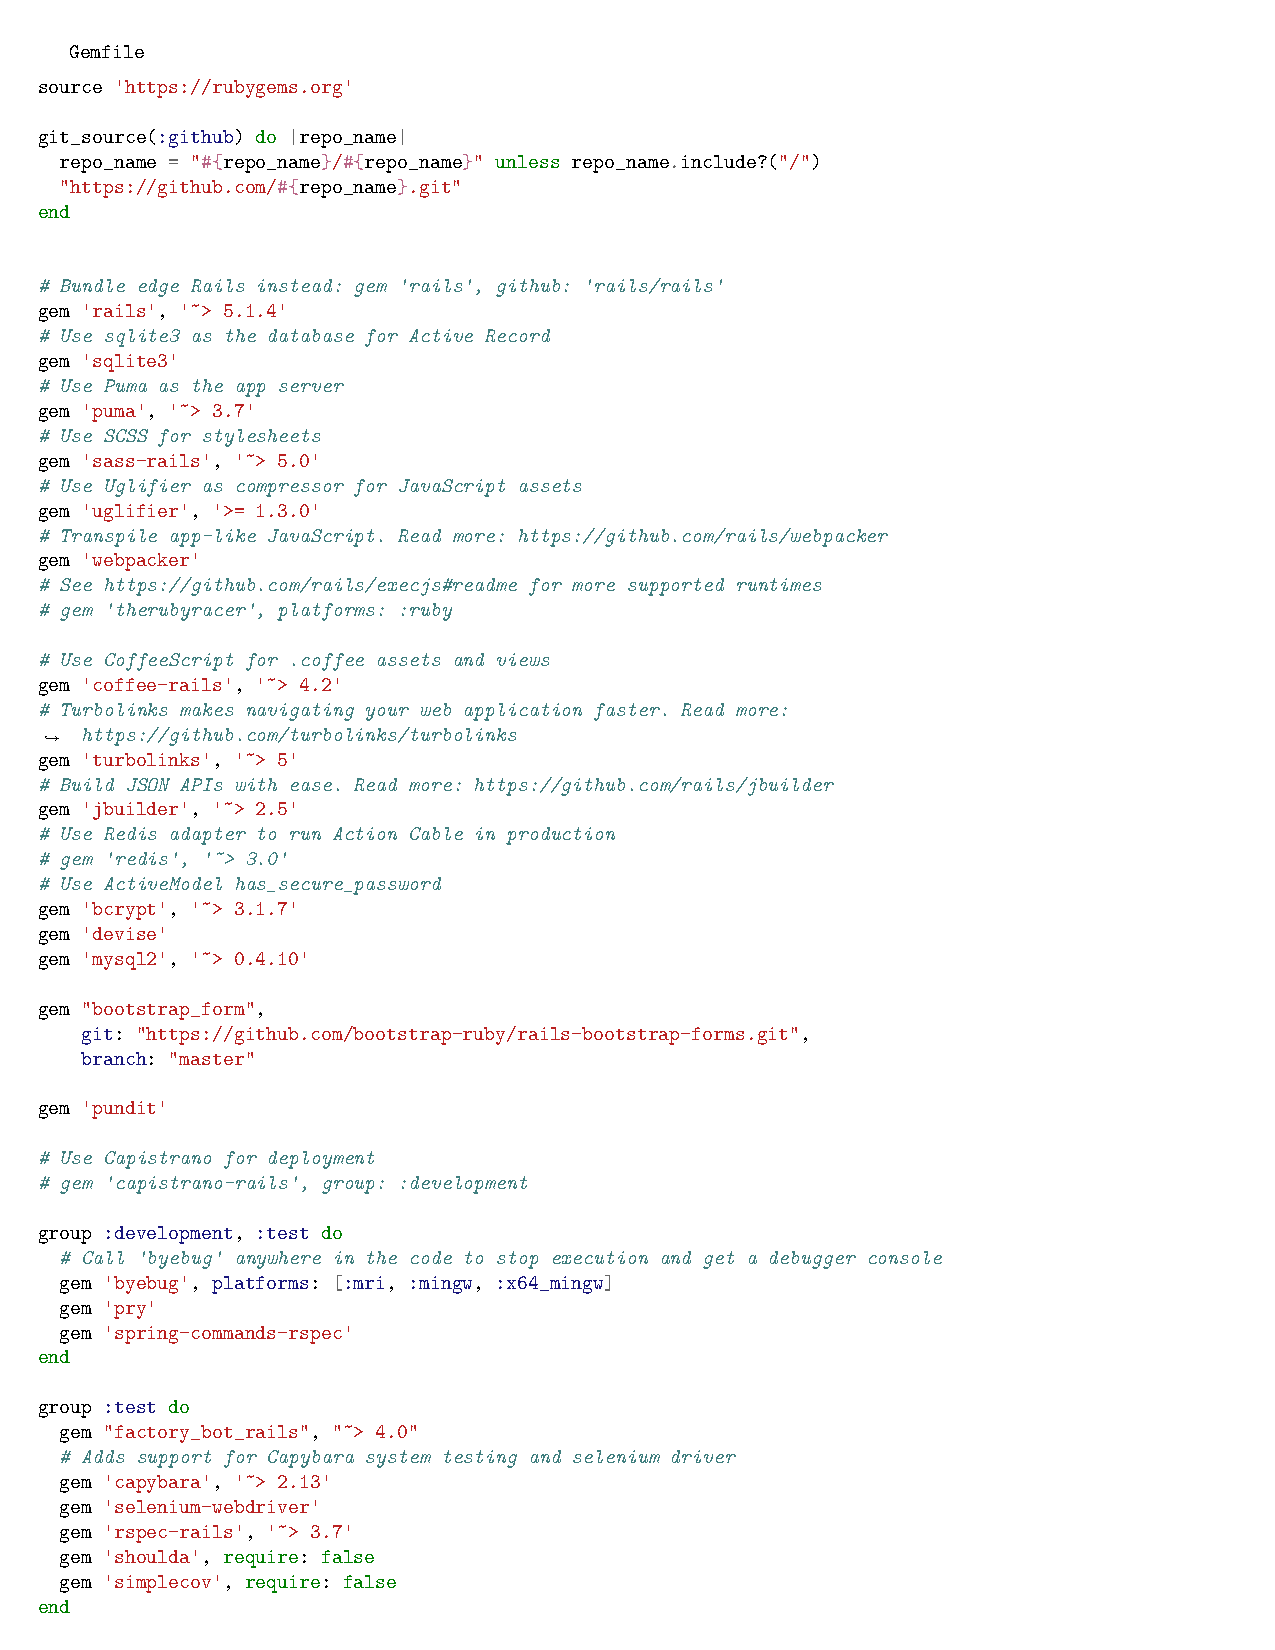
\includepdf[pages=1-72]{Appendices/sourcecodeweb.pdf}
\section{Code for sql parser}
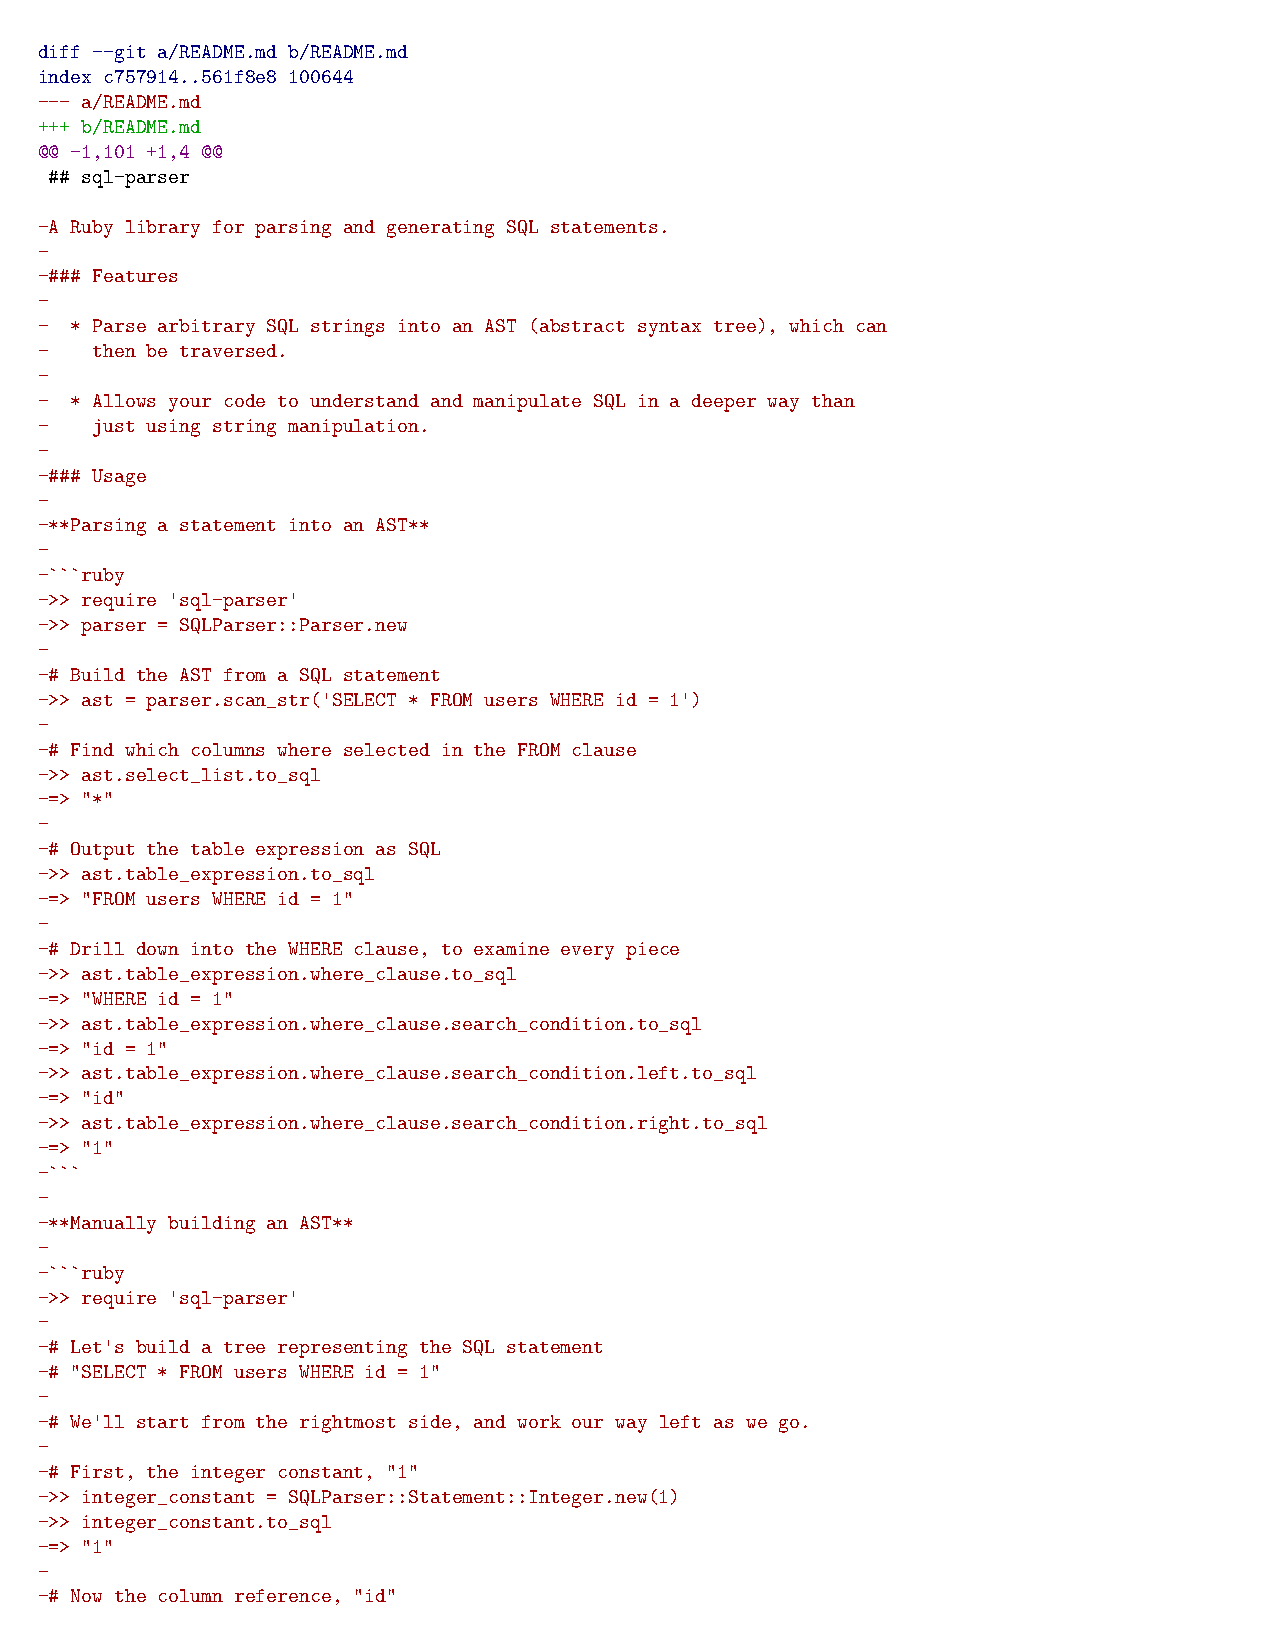
\includepdf[pages=1-7]{Appendices/sourcecodesql.pdf}
